This chapter will go more in depth about the several different kinds of hardware and software used. It will also elaborate on the different terms and names used for aspects of the research.
\section{$O^2$ Balancer}
$O^2$ Balancer is a framework used by CERN for simulation experiments for ALICE. The code is open source and licensed under the GNU General Public License V3.0. (GNU General Public License v3.0, 2007)

\subsection{Devices}
The $O^2$ Balancer consist of a cluster of 1750 computers, divided in 250 First Level Processors (FLPs) and 1500 Event  Nodes (EPNs) These computers are meant to process the data stream coming from ALICE. All of these computers are monitored using an Information Node.

\subsubsection*{First Level Processors}
The FLPs are the first computers in the line. They receive the data stream (approximately 1.1TB/s) from ALICE and need to distribute that to the next line of computer. In order to do that it takes the data received between two heartbeats, and compresses that into something that's called a Sub Timeframe (STF). A heartbeat lasts for about 20ms. It will then send this STF to the next line of computers which are the EPNs. Every EPN needs to get the same amount of STFs at the same time for recreation purposes. These STFs can then be further examined from there.("Technical Design Report for the Upgrade of the Online Offline Computing System", 2015, p. 33)

\subsubsection*{Event Processing Nodes}
The next line of computers are the EPNs. These receive the STFs from the FLPs and then compress them back into a time frame (TF). This compression reduces it's size by a factor of eight. These TFs are then stored for further use and examination.("Technical Design Report for the Upgrade of the Online Offline Computing System", 2015, p. 33)

\subsubsection*{Information Node}
There is one final computer which is the Information Node (IN). This computer keeps track of all the FLPs and EPNs that are online and makes sure that FLPs don't send data to offline EPNs. ("Technical Design Report for the Upgrade of the Online Offline Computing System", 2015, p. 34)

\begin{figure}
	\centering
	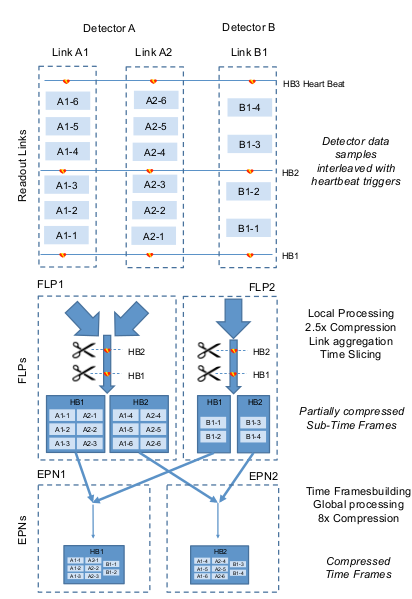
\includegraphics[scale=1]{./graphics/data_aggregation.png}
	\caption{Aggregation of data ("Technical Design Report for the Upgrade of the Online Offline Computing System", 2015, p. 34)}
\end{figure}

\section{FairMQ}
The transport layer used for the $O^2$ Balancer is FairMQ. This is a transport layer from the larger framework FairRoot \footnote{https://github.com/FairRootGroup/FairRoot} created by GSI Darmstadt. In order to accommodate the smaller processing size of the Raspberry Pi, a trimmed down version of FairRoot is used which is just FairMQ. This is a data transport layer used to send data in between the IN, FLPs and EPNs. 
\subsection{Splitting off FairMQ}
During this report, the FairMQ repository was split off from FairRoot. In the first stages of the prototype an emergency version was used made by Heiko van der Heijden. Meanwhile a pull request 
\footnote{https://github.com/FairRootGroup/FairRoot/issues/736} was done on the FairRoot github which resulted in the official FairMQ repository.

\section{Zookeeper}
Zookeeper is a program made by Apache to regulate the whole load balancing process. It is run on the Information Node and from there pings to all EPNs to check whether they are online or not. It then creates a list of online EPNs which it gives to the FLPs so that they know to what EPN to send data to. The frequency of these pings are called the Ticktime. 

\section{Fail-over}
When an EPN goes offline it is called a fail-over. When this happens, Zookeeper will know that it is offline and will notify the FLPs to not send any data to this specific EPN anymore. 

\section{Ansible}
Ansible is a deployment software used to create simple automation for large infrastructures. This is used to automate repetitive task for the experiment, and for deploying software stacks to every unit. 

\section{Blacklist Algorithm}
The algorithm used in the previous experiment is called a Blacklist Algorithm. This algorithm constantly keeps a list of ofline channels which is updated by the Information Node using Zookeeper. Once Zookeeper realizes that an EPN is offline, it will update the list so that the algorithm will skip that offline EPN. With this list of online EPNs, the algorithm uses a Round Robin approach to distribute the STF over the EPNs. A way to implement the Blacklist algorithm is shown in figure ~\ref{fig:BlacklistAlgorithm}

\begin{figure}[htb]
	\centering
	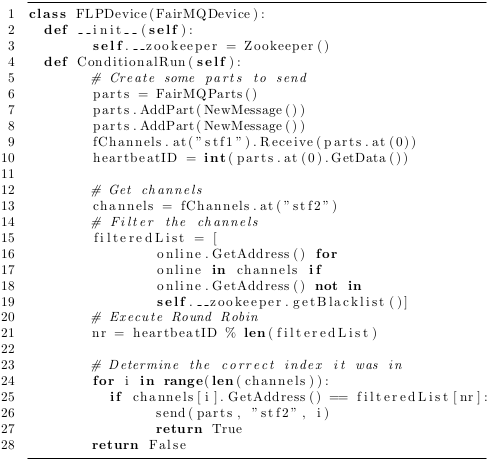
\includegraphics[scale=0.6]{./graphics/BlacklistAlgorithm.png}
	\caption{Blacklist algorithm as it could be implemented in Python (van der Heijden, 2018, p. 20)}
	\label{fig:BlacklistAlgorithm}
\end{figure}


\section{Raspberry Pi}
Raspberry Pi is a  low cost small computer used for prototyping projects \footnote{https://www.raspberrypi.org/about/}. These projects go from small sensor applications, to bigger host-server applications. The Raspberry Pi used for this research is the model 3 B+ variant. As of the time this report is written this is the latest version released. This model is used because of the high Ethernet speeds on the board itself. The reason a Raspberry Pi was used for this experiment is because it's a smaller and cheaper alternative compared to what the cluster on Nikhef used. (van der Heijden, 2018, p. 21) and because of this, it is more easily expanded.